\chapter{Simulation Experiments and Evaluation of the Architecture}
In this chapter, we present the results of simulation experiments developed to evaluate and explore choices offered by our K-HAS architecture. Using nodes with knowledge-processing capabilities to deliver interesting data quicker than a standard WSN, we have developed a simulation for our proposed architecture, K-HAS, as well as variations on the knowledge processing capabilities of the nodes at each tier.

The simulations were developed to determine whether K-HAS is the best mix of processing and collection nodes that maximises network lifetime while minimising the transmission time of interesting data. This was done by using a network structure, that matched our motivating scenario, and changing the knowledge-processing capabilities on each node at every tier; ranging from no knowledge on every node to the maximum knowledge-processing capabilities across the network. We aim to show that the more knowledge-processing capabilities that are pushed out towards the edge of the network, the more effective the network becomes at prioritising data that it believes to be interesting and delaying what it believes to be empty.

This chapter is structured as follows. Section \ref{sim:sim} describes the implementation of the network. Section \ref{sim:imp} outlines the results and Section \ref{sim:res} compares these with LORIS and the current solution in our motivating scenario. Section \ref{sim:conc} concludes our findings and highlights areas that require further experimentation.

\section{Simulation Environment}\label{sim:sim}

Using RePast Simphony \cite{Collier2003}, an agent-based network simulation tool developed in Java, we created a network to emulate K-HAS. RePast is an agent-based modelling system that allows for agents to be created and placed on a grid. Ticks denote a period of time and simulations can run for a fixed number of ticks, or until stopped. Ticks can also be used to schedule events, such as searching for neighbours, by calling methods that last for a set number of ticks, or begin at a particular tick. For example, a camera sensor node may be tasked with taking a picture every three hundred seconds. When the simulation reaches three hundred ticks (or six hundred, nine hundred, twelve hundred and so on), a scheduled event is run to simulate the camera's capture of an image and transmitting it to an endpoint.
%train may take three hundred for it to arrive at its destination. When the simulation reaches three hundred ticks, a scheduled event could run that would open the train doors, make an announcement and so on.

RePast was chosen because we did not require the low level network configuration provided by other tools, such as NS2 \cite{mccanne1997network}, but we did need to modify and record the behaviour between nodes as they capture and process sensed data. RePast's event scheduling allows for nodes to be modelled as agents and the dynamic configuration allowed us to modify the simulations during run time. The aim of these simulations was to visualise how different knowledge-processing capabilities can affect the prioritisation and transmission time of observations, as well as the accuracy of their classifications. RePast allowed us to utilise existing Java code we were using in our K-HAS middleware and develop a base simulation that could be configured easily with XML files.

Agents were created, using the RePast SDK, and Java classes were used to manipulate their behaviour. Simple networks may only contain basic agents with only a few variations from those provided by RePast. However, for more complex networks, a hierarchy of agents is required and Java's inheritance can then be used to create subclasses of an agent.

A 2D space is used to display the grid and the simulation is run within RePast's own GUI. This GUI provides functionality such as editing the properties of classes, integrating with Matlab, taking screenshots and saving different configurations of the same network.

\section{Experiment Design}\label{sim:imp}
	While the aim of these simulations was to show the effectiveness of K-HAS over the current solution, we also wanted to determine if it was the optimal solution, in terms of delivery of interesting data and network lifetime. We believe that the ideal solution would be to attach nodes with high knowledge-processing capabilities to all cameras in the network, however the short battery life means that replacements would be made as often as the current manual solution, detailed in Section \ref{tech:motiv}.

	Throughout this chapter, we will be referring to nodes tasked with different purposes as the three definitions listed here:
	\begin{itemize}
		\item Sensing Node: A node that has been tasked with the captuing, and routing, of sensed data.
		\item Routing Node: A gateway node that is tasked with collecting, processing and forwarding sensed data.
		\item Central Node: A node with similar functionality to a typical base station, tasked with storing all sensed data and providing an interface to users.
	\end{itemize}

	At the routing and sensing tier, the degree of knowledge processing capabilities can range from the levels outlined below:
	
	\begin{itemize}
		\item No Knowledge (NK): The node possesses no knowledge processing capabilities.
		\item Minimal knowledge (MK): The node possesses basic knowledge processing capabilities and contains a static rule base (Section \ref{khas:dc}).
		\item High Knowledge (HK): The node possesses high knowledge processing capabilities and is able to process data, metadata and use a dynamic rule base (Section \ref{khas:dp}).
	\end{itemize}
	
	The higher knowledge-processing capabilities of HK nodes allow them to classify observations with a greater accuracy, but their battery life is much shorter than MK nodes due to their increased power needs (Section \ref{tech:hw}). In contrast, MK nodes can run for a longer period without requiring battery replacement. MK nodes, however, are unable to classify observations to the same level as HK nodes. While HK nodes can classify an observation as interesting or empty and, in our scenario, match to a species, MK nodes can only assume an observation is interesting using the image's metadata as they lack the capabilities to reliably determine whether an observation is empty or not. The scenarios we have implemented cover combinations of HK, MK and NK, in a twenty five node network. We use twenty five nodes because DGFC had a between twenty and twenty two active cameras during our first and second visits and we knew that the first implementation of the network would require a single endpoint. From this, we chose to use four routing nodes so that each could handle an equal number of sensing nodes, if they were all within range, and a single central node. Our experiments in Danau Girang were restricted to a smaller number of nodes, due to cost, but we expected to deploy a sensing node onto all of the active cameras. The hierarchical nature of the network is shown in Figure \ref{fig:sim} and explained later in this section. These scenarios were developed to determine which combination of MK, NK and HK nodes allowed for the greatest network lifetime, as well as the greatest accuracy when delivering interesting sensed data, and they have been outlined below:
	
	\begin{itemize}
		\item NK-ALL: Sensing and routing nodes possess no knowledge processing capabilities.
		\item MK-ALL: Sensing and routing nodes possess minimal knowledge processing capabilities.
		\item NK-MK: Sensing nodes possess no knowledge processing and routing nodes have minimal knowledge.
		\item MK-HK (K-HAS): Sensing nodes have minimal knowledge and routing nodes possess high knowledge. This scenario matches the K-HAS architecture we proposed in Chapter \ref{chap:arch}
		\item HK-ALL: Sensing and routing nodes have high processing capabilities.
	\end{itemize}

Before implementing, we designed the agents required based on the nodes described in the ontology we proposed in Chapter \ref{chap:ont}. Using that, we created a hierarchy of nodes inheriting common properties from a node object. As previously mentioned, we had metrics on range and transmission times from previous experiments and the deployment of LORIS. We used these to create properties for each transmission medium that could be used by each node object. Table \ref{sim:tab:terms} shows how the K-HAS terms, introduced in Chapter \ref{chap:arch}, and LORIS terms, detailed in Chapter \ref{chap:imp}, map to the node types described above. The nodes used in our simulations map directly to the ontology.

\begin{table}[h]
\centering
\begin{tabular}{|l|l|l|}
\hline
\textbf{Network Type} & \textbf{Original Term} & \textbf{Maps To}          \\
\hline
K-HAS                 & DC Node                & Sensing Node + MK         \\
                      & DP Node                & Routing Node + HK         \\
                      & DA Node                & Central Node + HK         \\
LORIS                 & Buckeye                & Sensing Node + NK         \\
                      & DA and DP              & Routing/Central Node + HK \\
\hline
\end{tabular}
\caption{Mapping of K-HAS to Simulation Terminology}
\label{sim:tab:terms}
\end{table}

Using a Java library we developed for DwC archives during the implementation of LORIS (Section \ref{loris:arch}), we were able to implement DwC archives as the data standard in our simulations, this allowed us to model the prioritisation of sensed data, as well as the classification of observations, in the same way that a K-HAS deployment would.

The structure of the simulation is as follows: The \textit{network builder} instantiates all the nodes, places them randomly on the grid and schedules events once the simulation has started. The nodes then use the properties of their transmission medium to find nodes in range and create a connection; depicted by a line between the node. The simulation uses metrics, such as the size of the image, extracted from the images taken at Danau Girang and the chance of an image being captured by a camera is based on the average capture rate of a camera. The fire rate has been calculated by the average number of pictures captured in a day taken by each camera. Figure \ref{fig:sim} shows an example topology of the MK-HK scenario, sensing nodes are marked in yellow, routing nodes in green and the central node is red. Black edges are used to link the nodes. Each node is placed randmonly on the space and links are established between neighbouring nodes with the fewest hops to a central node. Network parameters are set in a configuration file, before the simulation runs, such as: the number of each node type and the size of the space.


	\begin{figure}[h]
	\centering
	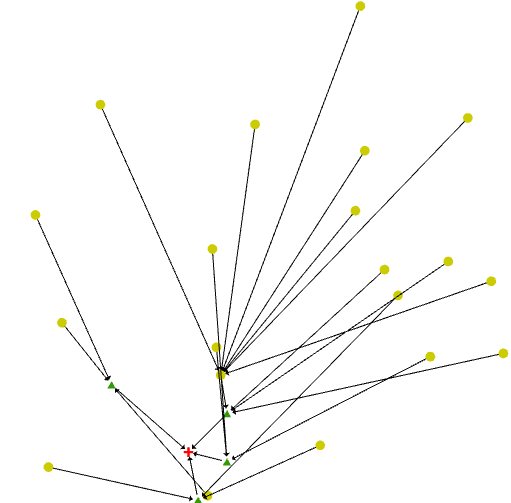
\includegraphics[width=0.8\textwidth]{Chap7/figures/khas_sim}
	\caption{MK-HK Simulation Example in RePast Simulator}
	\label{fig:sim}
	\end{figure}


%\begin{itemize}
%\item Network Builder
%\item Node
%	\begin{itemize}
%	\item Sensing
%	\item Routing
%	\item Central
%	\end{itemize}
%\item Darwin Core
%	\begin{itemize}
%	\item Identification
%	\item Location
%	\item Occurrence
%	\item Image
%	\item Species
%	\end{itemize}	 
%\end{itemize}

\subsection{Darwin Core}
The Darwin Core class represents a DwC archive, encapsulating \textit{Identification}, \textit{Location}, \textit{Occurrence}, \textit{Image} and \textit{Species} (Section \ref{buildcapture}). The images we have collected from Danau Girang were processed to find details such as the average size when captured at night and day, how often an average camera triggers and the percentage of images with animal content. These data were then used to specify how often a randomly placed node should capture an observation per tick.

Upon each capture, images are created and given a random size, between the maximum and minimum size found in the 120,000 images collected from DG. The sum of the image sizes is used to calculate the size of the archive. Using this size, a sensing node calculates how long the archive takes to send based on the size and the transmission rate. We assume that the rate stays constant for the duration of transmission.
When an archive is sent to the routing node, we used the average time for our image processing tool and Drools engine to run and attempt a classification, which is 43 seconds (ticks), explained in detail in Section \ref{tech:sf:triton}. To keep the classifications as general as possible, so that the simulation applies to any WSN for scientific observations, archives are not classified down to the species level, they are marked as \textit{interesting} or \textit{empty} and then forwarded to the central node.

\subsection{Routing}
The routing protocol used needs to be dynamic in order to adapt to nodes being added and removed during deployment, while minimising traffic in a resource constrained network. In our approach, we use a modification of the Minimum Cost Forwarding Algorithm (MCFA), described in Section \ref{arch:routing}. A cost is assigned to each node, based on how far they are from the central node, with neighbouring nodes choosing to connect to the node with the lowest cost. However, in normal implementations of MCFA, all nodes are of the same type and simply need to connect to a central node. This protocol is used in all scenarios.

In our K-HAS architecture, sensing nodes cannot connect directly to a central node because processing would not take place. Because of this, we used the same routing method across all scenarios. Our implementation of MCFA works with a discovery phase and a transmission phase. The discovery phase is a scheduled event, taking place at the start of deployment but it can be run throughout deployment to react to nodes being added or removed. 

\subsubsection{Discovery}\label{sim:disc}
	Discovery begins at each central node, scanning nodes in range for routing nodes and sending a broadcast packet, with a cost of 0, to inform them that they are within range of a central node. Links between Central and Routing nodes use W-Fi in all of our scenarios. Once received, routing nodes increment the count and forward the packet to any routing nodes within range of them, where we use the range of Zigbee. We found that this method overloaded the routing nodes and all sensing nodes within range would connect to the first routing node they receive the broadcast from. We then implemented a method, called \textit{load balancing} \cite{Gupta2003}, which uses the sensing nodes connected to a routing node to calculate whether it should offload new nodes to a neighbouring routing node.
	
	The maximum connections a routing node can have is determined by the total number of sensing nodes in the network divided by the total number of routing nodes, which is held in the knowledge base of the central node. Once a routing node has the maximum number of connections allowed, it starts to offload to a neighbouring routing node that is also in range of the sensing node requesting a connection. If there are no neighbouring nodes then the routing node exceeds the maximum number of connections allowed, to save sensing nodes being left with nowhere to send their data.
	
	If the sensing node that receives the broadcast does not have an existing route to a central node, or the cost of the current route is higher than the received route, it adds an edge to the routing node, increments the count and forwards it to all nodes in range. This process continues until the broadcast reaches the edge of the network. Nodes do not have global knowledge of the route to the central node, only of their neighbour with the lowest cost.
	
	This phase can be repeated throughout the course of the deployment, simply by scheduling it as an event to occur every \textit{n} ticks. However, the simulation currently only uses the discovery phase at the beginning of the deployment.
	
\subsubsection{Transmission}
	Once the discovery phase has been completed, providing nodes are within range of the central node, the transmission phase begins where only DwC archives are then sent across the network. Observations are captured based on the mode of the simulation and sent to the lowest cost neighbour.
	
	In order to manage transmissions, sensing nodes have a \textit{SendState} object that contains the next archive to send, the time to send it and whether it is currently sending. This is used to determine what operations to perform, once an archive has been sent, it is deleted from the SendState and the sending flag is set to false. A new archive is then added and sent when the opportunity arises.
	
	When a routing node receives the archive, it begins processing. Routing nodes use the SendState as well, but they only add an archive once it has been processed and they then select the oldest archive that has been classified as interesting, providing an archive is not already waiting to be sent. The archive stores information about the route it takes, recording every hop, as well as the time it took from capture to central node.
	
	Scheduled sending events run every thousand ticks, which is configurable, to check the sending state of the node and send any archives in the SendState. The node then waits for the number of ticks that it will take in order to transmit the archive.
	
	Once the simulation is completed, either manually or through a defined number of ticks, the archives in each central node are iterated over and written to a CSV file, with details such as the path it took, total transmission time and time of capture.
	
\subsection{Capture}
	Using the existing data collected from Danau Girang, we calculated how often a camera triggers in a six month deployment, as well as how often the observation contained interesting content. 
	
	To calculate the count of interesting images, we processed every directory of images to extract the largest object in the foreground, using our Triton program. Once processed, we iterated through every directory, counted the total number of images and the total number of extracted images; an extracted image is a black and white image containing the largest object that has been found in the observation and are only created when the processing believes that the observation is interesting. This gave us a 20.7\% chance of an image being interesting, across every camera.
	
	The chance of a camera being triggered each second was calculated by the total number of observations (13,399) divided by the number of seconds in six months (15,552,000). This gives a chance of 0.000861561 of a camera trigger in any given second.
	%Edit this to explain why it runs every 1000 ticks
	
\subsection{Processing}
	The types of knowledge processing capabilities that we outlined in Section \ref{sim:imp} are used in the simulation to determine which type of processing to perform on observations. The result of processing is that an observation is marked as interesting or empty. The limitation of our image processing tool is that only the largest region of interest (ROI) is extracted, even if there are multiple objects in the image. The outcome can be any of the following:
		\begin{description}
			\item True positive (TP): An ROI is extracted that contains the animal in the set.
			\item False positive (FN): An ROI is extracted that contains nothing of interest.
			\item True negative (TN): A camera is triggered with nothing of interest in the image and no ROI is extracted.
			\item False negative (FN): An image containing an animal has no ROI extracted.
		\end{description}
	
	Using the results of our image processing application (explained in Section \ref{tech:sf:triton}) for the properties of HK processing, we encoded that an 82\% accuracy at detecting TP images, with a 98\% accuracy for finding TN images. Nodes with MK do not have the ability to mark an image as empty, but they can mark an image as interesting. However, the results we have from our rule base are not as extensive as the results we have for Triton (due to limited local knowledge and existing rules approved by domain experts), so instead we use a predefined 10\% accuracy for detecting TPs. This 10\% is used because we needed to show the difference between a node with MK and a node with HK. HK nodes have the ability to process the contents and metadata of sensed data, with access to libraries and a dynamic knowledge base. MK nodes are able to look at the basic metadata and only have a static knowledge base, limited in size. In future work, we could test with greater accuracy or, with more rules, we could run experiments to find the exact accuracy of an MK node. An interesting image is an image that contains an animal and can be either a TP or FN. Empty images are those that do not contain an animal and can be either FP or TN.
	

\section{Results}\label{sim:res}
In this section, we explains the results from simulating each scenario in a randomly generated network graph. 

Each scenario, outlined in Section \ref{sim:imp}, runs to simulate a 6 month deployment. Using our motivating scenario, we modelled each scenario on a fixed number of nodes: 1 central node, 4 routing nodes and 20 sensing nodes. The implementation of our architecture has been limited to using Zigbee as the transmission medium between all sensing nodes, with a Wi-Fi connection between routing nodes and a central node. Sensing nodes then send an observation when it is captured or, if it has not captured anything then it checks for a backlog every ten minutes. Sensing nodes check for new observations to process every five minutes. We ran each scenario a hundred times, with each run simulating a 6 month duration. The time to process an observation using MK has been simulated to take 5 seconds compared to the 43 seconds when a node has HK capabilities; these values have been chosen based on the average processing time we derived using existing data. 

\begin{figure}[ht!]
	\centering
	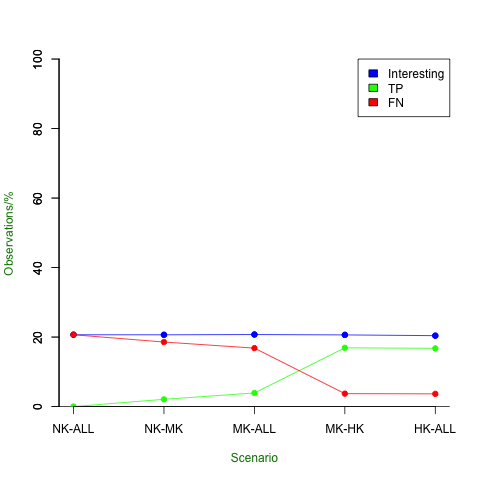
\includegraphics[width=0.8\textwidth]{Chap7/figures/ideal/all_int_percent}
	\caption{Percentage of Interesting Observations for All Scenarios.}
	\label{fig:res:ideal:int}
\end{figure}

The simulations were run in two modes: ideal transmission rate and variable transmission. Ideal used a fixed transmission rate (250kbps) for Zigbee links between all sensing nodes, with all observations being sent at the highest possible rate. Variable generates a random number for the transmission rate (between 20 and 250kbps) for each sensing node link, at the time of the network's initialisation. This models the large fluctuations in both speed and range that we observed in the Malaysian rainforest when we ran tests with Zigbee equipment. The Wi-Fi range remains constant because the distance of routing nodes from central nodes, in our motivating scenario, can be made small enough that a consistently good connection is achievable.

\begin{figure}[ht!]
\centering 
\begin{subfigure}{0.8\textwidth}
  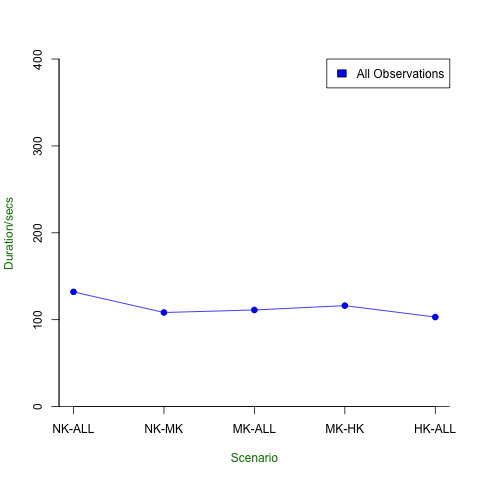
\includegraphics[width=0.8\textwidth]{Chap7/figures/ideal/all_total}
	\caption{Ideal Transmission Rates.}
	\label{fig:res:ideal:dur}
\end{subfigure}
\begin{subfigure}{0.8\textwidth}
  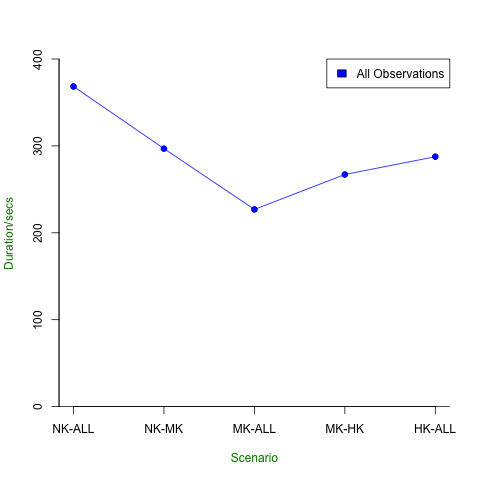
\includegraphics[width=0.8\textwidth]{Chap7/figures/real/all_total}
	\caption{Variable Transmission Rate.}
	\label{fig:real:dur}
\end{subfigure}
\caption{Mean Duration of All Observations}
\label{fig:mean:dur}
\end{figure}

Figure \ref{fig:res:ideal:int} shows the percentage of interesting observations that arrive at the central node. Due to the short transmission time, almost all observations arrive in near real-time (fewer than 2 minutes) and, as such, the split between empty and interesting remains almost constant at approximately 80:20. This is important because the chance of an image being interesting is 20.7\%, so all data is being received at the DA node, without any observations backed up on nodes in the network. However, the True Positive observations are the most important as they are the interesting observations that have been marked as such. False Positives are interesting observations that have been wrongly marked as empty. Increasing the knowledge processing capabilities of routing nodes, shown by the difference between MK-ALL and MK-HK, increases the number of TPs, as well as reducing the number of FPs. Another important point to note is that MK-HK and HK-ALL provide the same results, despite HK-ALL solely consisting of nodes with the highest knowledge processing capabilities.  This is probably due to the fact that all observations, in MK-HK, go through an HK routing node and, thus, would receive the same level of processing as in an HK-ALL scenario.

These results support our hypothesis that MK-HK is the best scenario to choose in terms of timeliness of data delivery, quality of data delivered and network lifetime, as MK-HK has all sensing nodes with minimal knowledge processing capabilities, allowing them to run for approximately three months, achieved from tests detailed in Section \ref{tech:hw:conc}. However, with HK-ALL, all sensing nodes run with higher capabilities and are limited to run for a maximum of three weeks before battery replacement is required. While this number is similar to the current, manual process described in Section \ref{tech:motiv}, this does include processing and prioritisation of sensed data, which can take weeks or, sometimes, months when carried out by humans.

\subsection{Duration}
The ideal transmission rate runs with the transmission rates of all nodes at their theoretical maximum, giving the highest speed for both Zigbee and Wi-Fi. Figure \ref{fig:res:ideal:dur} shows the mean duration of any observation, interesting or empty, in each scenario. With the exception of NK-ALL, it is clear scenarios that, where more nodes have higher knowledge processing capabilities, the mean duration is increased. An explanation for NK-ALL nodes showing a higher average duration is because the lack of knowledge on any of the nodes prevents it from prioritising observations, which means that some could be queued for longer before being sent on. One of the key points to note is that the difference in transmission time from capture to central node is typically no more than one hundred seconds. When compared with a standard, power efficient WSN with no knowledge processing capabilities, the reduced battery life may not be worth the trade off. However, these times are not solely for transmission, they also include in-network processing and prioritisation when they arrive at the central node. 

\begin{table}[h]
\centering
\begin{tabular}{|l|l|l|l|l|l|}
\hline 
      & Total & Interesting & \% Interesting & Empty & \% Empty \\
\hline
NK-ALL & 44205 & 9133        & 20.7           & 35071 & 79.3     \\
NK-MK  & 44244 & 9136        & 20.6           & 35107 & 79.4     \\
MK-ALL & 44052 & 9132        & 20.7           & 34920 & 79.3     \\
MK-HK  & 43754 & 10066       & 23.0           & 33688 & 77.0     \\
HKALL & 42511 & 9671        & 22.7           & 32840 & 18.9     \\
\hline   
\end{tabular}
\caption{Mean Number of Observations for All Scenarios under Ideal Transmission Rate}
\label{sim:tab:ideal}
\end{table}

During our visits to Danau Girang, we performed experiments for many different transmission methods: Wi-Fi, Zigbee and RF. The results were always different to what we experienced in the UK and the variation in connectivity in just a few minutes, or metres, was extreme in some cases. Days where the humidity was one percent higher than the previous day could result in a 50\% range drop and rain for a few minutes could drop all connections for an hour afterwards. Modelling this in our simulations was necessary to accurately plan for what we could expect in Malaysia. Our planned network topology (Section \ref{arch:scen}) in Danau Girang has routing and central nodes so close to each other that the Wi-Fi connection remained fairly stable and connectivity should remain at 100\%. When simulating sensing nodes, we randomly set their transmission rate between 20 and 250kbps at the start of each run. As each scenario is being run 100 times, this method is more efficient while still allowing for variation in the transmission rates. 

The number of interesting observations received in each scenario remained similar to the ideal mode (see Tables \ref{sim:tab:ideal} and \ref{sim:tab:variable}), as expected, but the fluctuation in transmission time (Figure \ref{fig:real:dur}) is much larger, with some images taking 800 seconds, or 13 minutes. In our motivating scenario, this is not much of an issue. However, if the image was of a hunter or the scenario was building intrusion detection system, then thirteen minutes is a long delay that could cause considerable damage. Of course, using all Wi-Fi connections is a more feasible option, but situations where long range is required prevents this. Our simulations do not currently take into account broken links in the network, where changes to the node's environment (such as a fallen tree) could cause it to drop out of range for a few minutes, or even hours, but this can be addressed by implementing the discovery phase (described in Section \ref{sim:disc}) of the routing protocol to run at a set interval throughout the duration of the simulation.

The duration of an observation with both a variable and ideal transmission rate does not fluctuate largely and Figure \ref{fig:res:ideal:int} shows that the processing power of MK-HK vs. HK-ALL is identical. However, Figures \ref{fig:real:int:dur} and \ref{fig:real:empty:dur} show that the primary benefit of pushing HK processing capabilities out to the edge of the network allows for better prioritisation of observations. Sensing nodes with HK are able to determine whether an observation is interesting or empty with much greater accuracy than MK and these capabilities, right at the edge of the network, allows for an interesting observation to be processed as soon as it is captured and sent without further processing directly to a central node. The only delays being the processing time itself and the sending queue of intermediate nodes. Figures \ref{fig:real:int:dur} and \ref{fig:real:empty:dur} show that, when a network is not saturated, interesting and empty observations take a similar amount of time to pass through the network; with the exception of the HK-ALL scenario. WSNs with much worse transmission rates could experience a much larger time difference between interesting observations, especially when using long range FM frequencies that can transfer only a few bytes a second.
\begin{figure}[ht!]
\centering
    \begin{subfigure}{0.8\textwidth}
	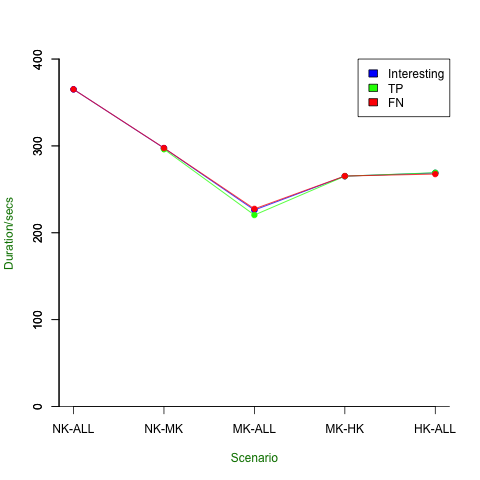
\includegraphics[width=0.8\textwidth]{Chap7/figures/real/all_int}
	\caption{Interesting Observations.}
	\label{fig:real:int:dur}
	\end{subfigure}	

	\begin{subfigure}{0.8\textwidth}
	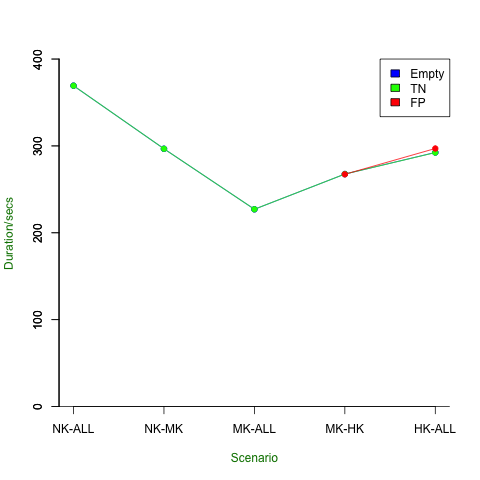
\includegraphics[width=0.8\textwidth]{Chap7/figures/real/all_empty}
	\caption{Empty Observations.}
	\label{fig:real:empty:dur}
	\end{subfigure}	
\caption{Mean Duration under Variable Transmission Rate}
\end{figure}

\begin{table}[h]
\centering
\begin{tabular}{|l|l|l|l|l|l|}
\hline
      & Total & Interesting & \% Interesting & Empty & \% Empty \\
\hline
NK-ALL & 43743 & 9012        & 20.6           & 34730 & 79.4     \\
NK-MK  & 44258 & 9195        & 20.8           & 35063 & 79.2     \\
MK-ALL & 44152 & 9130        & 20.7           & 35021 & 79.3     \\
MK-HK  & 44273 & 10183       & 23.0           & 34059 & 77.0     \\
HK-ALL & 43011 & 9935        & 23.1           & 33076 & 18.9     \\
\hline
\end{tabular}
\caption{Mean Number of Observations for All Scenarios under Variable Transmission Rate}
\label{sim:tab:variable}
\end{table}

\subsection{Network Saturation}



With the transmission rates of Zigbee and Wi-Fi, an observation of three images, each under a megabyte in size, can be processed and sent in a matter of minutes; when there are only a few hops. However, with these network topologies, we are unable to see how each scenario handles prioritisation when it is unable to send every observation captured. This can be done by either reducing the transmission rate or increasing the chance of an observation being captured. We chose to increase the chance of an observation being captured and maintaining the transmission rate in order to keep the simulations in line with our motivating scenario. Existing data from Danau Girang has shown a seasonality change in the number of images captured and we know that some sites are more active than others, therefore making a higher chance of capture more fitting. 

Imagine a scenario where flash floods in the rainforest prevent access to the nodes to change the battery and a mating season of sun bear has caused the capture rate to increase. The chance of an image capture has increased and users of the network have programmed the sensing nodes's sleep duration to a minute; saturating the network with more images than can be sent in a six month period.

\begin{table}[h]
\centering
\begin{tabular}{|l|l|l|l|l|l|}
\hline
      & Total  & Interesting & \% Interesting & Empty  & \% Empty \\
\hline
NK-ALL & 254352 & 127149      & 50           & 127149 & 50     \\
NK-MK  & 264580 & 144058      & 54.4         & 120522 & 45.6     \\
MK-ALL & 183727 & 126530      & 68.9           & 57196  & 31.1     \\
MK-HK  & 159446 & 115054      & 72.2           & 44392  & 27.8     \\
HK-ALL & 192010 & 155656      & 81             & 36353  & 18.9     \\
\hline
\end{tabular}
\caption{Mean Number of Observations for All Scenarios when Saturated}
\label{sim:tab:satur}
\end{table}

We simulated this across all five scenarios and the results are detailed in this section. The duration is increased for all observations (Figure \ref{fig:sat:total:dur}) and there is an increase in the time it takes an interesting observations when compared to an empty observation. Table \ref{sim:tab:satur} shows the average number of observation captured across all scenarios, however, when you look at the number delivered, we can see that the number of interesting observations delivered is much greater. This means that the network is successfully prioritising observations it believes to be interesting and not sending those that are empty because of the time and bandwidth constraints.

	\begin{figure}[ht!]
	\centering
	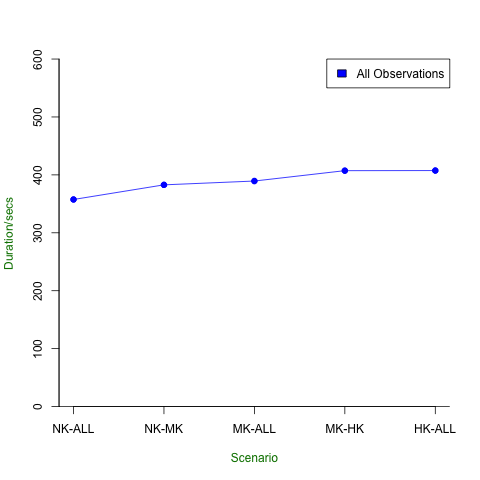
\includegraphics[width=0.8\textwidth]{Chap7/figures/saturated/all_total}
	\caption{Mean Duration of All Observations Across All Scenarios}
	\label{fig:sat:total:dur}
	\end{figure}

Figure \ref{fig:sat:total:dur} shows that the mean transmission time of all observation does not differ much between scenarios (with all scenarios at approximately 400 seconds) when the network is saturated, but we can see that the network must decide what images to send or drop when there are more observations than bandwidth available. HK-ALL is the slowest of these because of the increased time it takes to process and image with HK. This is shown more clearly when we compare \textit{interesting} and \textit{empty} observations. The red line (showing false positives) only exists for MK-HK and HK-ALL scenarios because MK nodes are not able to classify an observation as empty and, as such, NK-ALL, NK-MK and MK-ALL do not generate any false positives.

	\begin{figure}[ht!]
	\centering
		\begin{subfigure}{0.8\textwidth}
		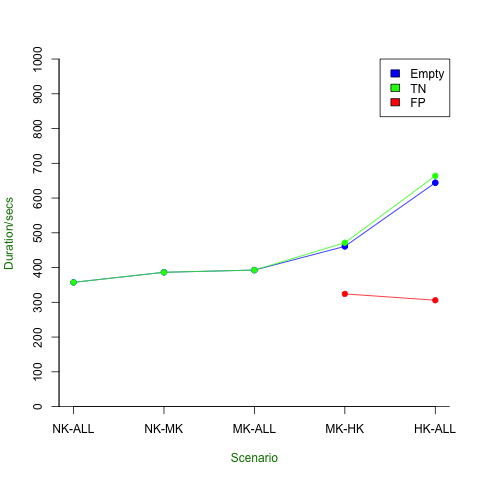
\includegraphics[width=0.8\textwidth]{Chap7/figures/saturated/all_empty}
		\caption{Empty.}
		\label{fig:sat:empty:dur}
		\end{subfigure}

		\begin{subfigure}{0.8\textwidth}
		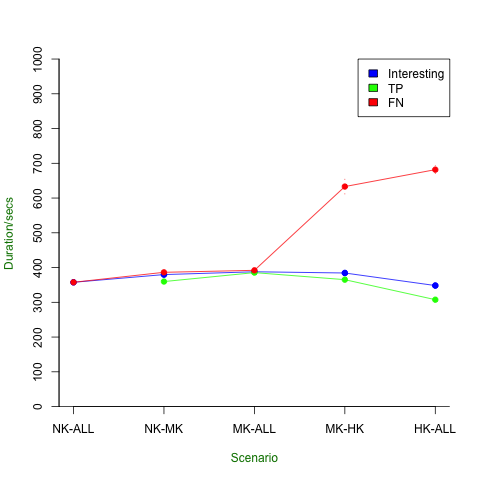
\includegraphics[width=0.8\textwidth]{Chap7/figures/saturated/all_int}
		\caption{Interesting.}
		\label{fig:sat:int:dur}
		\end{subfigure}
	\caption{Mean Duration of Observations across All Scenarios}
	\end{figure}

The mean transmission time of empty images (Figure \ref{fig:sat:empty:dur}) shows that the increase of knowledge processing capabilities improves the network's ability to filter out empty observations and a network with only HK nodes is able to defer empty observations from the time of capture so that bandwidth remains free for those that are interesting. Figure \ref{fig:sat:int:dur} shows the mean transmission time of interesting observations and we can see that interesting observations misclassified as empty bring the average duration for interesting observations up to approximately 400 seconds but the ability to prioritise allows TP observations to be delivered at a much faster rate of between 300 and 400 seconds, compared to more than 800 seconds for empty observations. It is worth nothing that, while misclassified interesting observations (FP) take longer to reach the central node in higher knowledge scenarios, the number of them received is greatly reduced from between 30\% and 45\% in MK scenarios to less than 20\% for HK scenarios; as shown in Figure \ref{fig:sat:int:percent}.

	\begin{figure}[ht!]
	\centering
	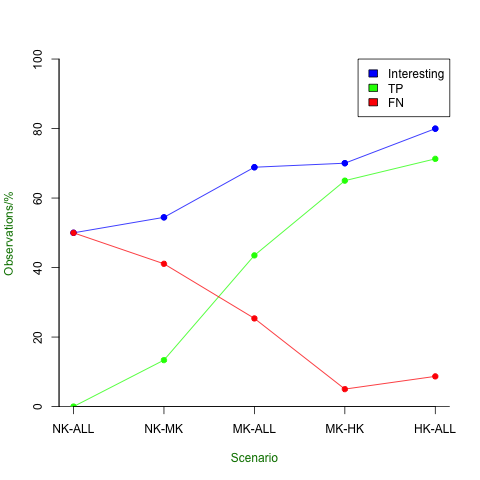
\includegraphics[width=0.8\textwidth]{Chap7/figures/saturated/all_int_percent}
	\caption{Percentage of Interesting Observations across All Scenarios}
	\label{fig:sat:int:percent}
	\end{figure}

	\begin{figure}[ht!]
	\centering
	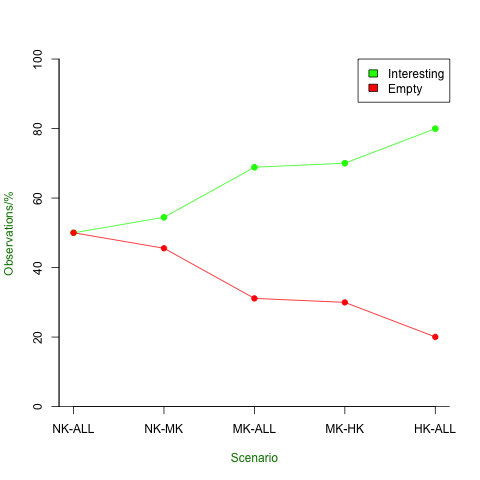
\includegraphics[width=0.8\textwidth]{Chap7/figures/saturated/all_int_empt}
	\caption{Percentage of Interesting Compared to Empty Observations across All Scenarios}
	\label{fig:sat:int:empty}
	\end{figure}

Saturating each scenario shows how different levels of knowledge processing across the nodes can prioritise the delivery of interesting observations while filtering out observations that have been classified as empty. We can see that the HK-ALL scenario delivers the highest percentage of interesting observations (80\%), with a slightly higher average transmission time. Having HK on all nodes causes a large reduction in the lifetime of the network to 3 weeks. MK-HK (or K-HAS) is a good alternative to this as it provides a network lifetime of 3 months for the majority of the nodes but still around 70\% of all images (same as MK-ALL) are interesting, but the majority of these are \textit{true positives}. In a network with limited access to a power source, MK-HK is the best implementation but, for networks with access to a continuous power source, HK-ALL can be used to increase the number of interesting observations delivered to the central node in a shorter time period.

% \subsection{Scenarios}

% This section details the results from each scenario of increasingly capable knowledge processing nodes. NK-ALL represents a 'standard' WSN where no nodes have knowledge processing capabilities and forward to a single endpoint. NK-MK simulates a network where sensing nodes have no knowledge processing capabilities, but routing nodes have MK, allowing them to detect whether an observation is interesting, but lack the knowledge to determine, with any confidence, whether an observation is of no interest. MK-ALL simulates a network where both sensing and routing nodes have MK capabilities. MK-HK is the RePast implementation of our K-HAS architecture; sensing nodes have MK and routing nodes have HK. HK-ALL has sensing and routing nodes that have HK capabilities. 

% Table \ref{tab:observ_int} shows the time for average transmission time, in hours, for interesting observations. Interesting observations consist of \textit{true positives} and \textit{false negatives}, which means that the spread of transmission times would be quite varied, because TPs would be prioritised but FPs would be treated as empty images. However, we can see that the total of interesting images almost doubles when all nodes have HK. More importantly, the difference between HK-ALL and MK-HK is less than 2\%, while still providing a battery advantage. With MK-HK and HK-ALL, the median is much lower when compared to MK-ALL and NK-MK, due to the higher levels of knowledge processing capabilities.

% With the results broken down further, Table \ref{tab:observ_tp} shows the average duration for true positives and we can see that, while the median stays much the same for each scenario, average duration varies considerably. The average time for a TP to be sent is lower for MK-HK than for MK-ALL, this could be due to the extra processing time for HK nodes or a processing backlog with a large number of observations. Although the duration of MK-HK is approximately twice that of MK-ALL, it does deliver more TPs, with 36.46\% of all images received being TP, compared with 8.45\% for MK-ALL.

% \begin{table}[h]\footnotesize
% \begin{tabularx}{\textwidth}{ |X|X|X|X|X|}
% \hline
% Scenario & Median & Mean & Standard Deviation & \% Total\\
% \hline
% NKMK & 608 & 841.95 & 854.18 & 22.11\\
% MKALL & 127 & 652.33 & 868.09 & 24.35\\
% MKHK & 3 & 255.49 & 591.63 & 38.86\\
% HKALL & 2 & 59.57 & 320.48 & 40.78\\
% \hline
% \end{tabularx}
% \caption{Transmission Time for Interesting Observations}\label{tab:observ_int}
% \end{table}

% \begin{table}[h]\footnotesize
% \begin{tabularx}{\textwidth}{ |X|X|X|X|X|}
% \hline
% Scenario & Median & Mean & Standard Deviation & \% Total\\
% \hline
% NK-MK & 3 & 277.01 & 543.22 & 3.88\\
% MK-ALL & 2 & 99.73 & 353.16 & 8.45\\
% MK-HK & 3 & 207.09 & 518.11 & 36.46\\
% HK-ALL & 2 & 2.77 & 2.75 & 38.16\\
% \hline
% \end{tabularx}
% \caption{Transmission Time for True Positive Observations}\label{tab:observ_tp}
% \end{table}

% \begin{table}[h]\footnotesize
% \begin{tabularx}{\textwidth}{ |X|X|X|X|X|}
% \hline
% Scenario & Median & Mean & Standard Deviation & \% Total\\
% \hline
% MK-ALL & 675.5 & 945.94 & 916.11 & 15.9\\ 
% MK-HK & 683 & 989.02 & 1006.4 & 2.41\\
% HK-ALL & 553 & 885.65 & 931.19 & 2.6\\
% \hline
% \end{tabularx}
% \caption{Transmission Time for False Negative Observations}\label{tab:observ_fn}
% \end{table}

% \begin{figure}[!h]
% \centering
% 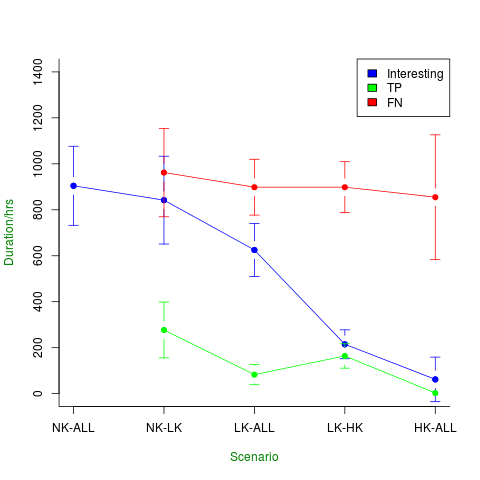
\includegraphics[width=\textwidth]{Chap7/figures/all_int.png}
% \caption{Mean Transmission Time for Interesting Observations in All Scenarios}
% \label{fig:all_int}
% \end{figure}

% \begin{figure}[!h]
% \centering
% 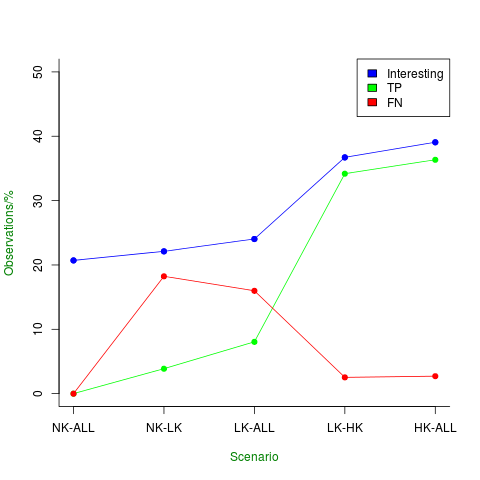
\includegraphics[width=\textwidth]{Chap7/figures/all_int_percent.png}
% \caption{Percentage of Interesting Observations in All Scenarios}
% \label{fig:all_int_percent}
% \end{figure}

% Figure \ref{fig:all_int} shows the average transmission time for interesting observations across every scenario. NK-ALL has no points for TP and FN because of its lack of processing capabilities. The drop in transmission time for interesting images is clearly visible here, but there is an increase in TN transmission time when comparing MK-ALL and MK-HK. This spike is better explained with the use of Figure \ref{fig:all_int_percent}, showing that, although it takes longer for TP images to be delivered in MK-HK, the percentage of TP images increased in MK-HK by almost four times that of MK-ALL. The faster transmission times in HK-ALL can be explained by the fact that all nodes can accurately detect empty images from the edge of the network and also prioritise interesting images with a greater accuracy than any other scenario. However, nodes with HK processing power have much higher power requirements and require battery changes every 3 weeks, this power trade off shows that nodes of this type can deliver interesting observations significantly faster than nodes with MK. A number of WSNs will place nodes in places that are not easily accessible by humans and not expected to be visited so regularly. In our motivating scenario, some nodes could be rendered inaccessible by river floods for weeks at a time and regular human traffic can prevent animals from using those sites. The percentage of TPs delivered by MK-HK and HK-ALL are not that different, but the delivery time when using both HK and MK nodes does affect the delivery time. 

% \subsection{MK-HK Scenarios}

% The main difference between HK-ALL and MK-HK is that all sensing nodes in HK-ALL have the ability to perform more intense data processing and determine which observations to prioritise with greater accuracy. Whereas MK-HK focusses on HK capabilities for the routing nodes and maximising the lifetime of sensing nodes by limiting them to MK capabilities. Therefore, we tested different proportions of MK and HK sensing nodes within the MK-HK scenario in order to determine the best ratio between performance and network lifetime. Table \ref{tab:khas_int} shows the average duration for an interesting observation when 4, 8, 12, 16 and 20 of the 20 sensing nodes have HK, with the rest having MK processing capabilities. Figure \ref{fig:khas_int_percent} illustrates how pushing knowledge further towards the edge of the network increases the delivery time and the percentage of interesting images. MK-HK 16 and MK-HK 20 have an average difference of three hours for interesting images, but MK-H K20 means that all nodes in the network have HK processing capabilities and, thus, a shorter battery life. While the difference in transmission time is not that significant, the extra MK nodes with a longer battery life means that they can be placed in areas that may not be easily accessible or need to remain undisturbed.

% \begin{table}[h]\footnotesize
% \begin{tabularx}{\textwidth}{ |X|X|X|X|}
% \hline
% Scenario & Median & Mean & Standard Deviation \\
% \hline
% MK-HK 4 & 2 & 153.21 & 462.75 \\
% MK-HK 8 & 2 & 146.04 & 428.79 \\
% MK-HK 12 & 2 & 156.95 & 461.67 \\
% MK-HK16 & 2 & 88.86 & 349.68 \\
% MK-HK 20 & 2 & 63.13 & 330.67 \\
% \hline
% \end{tabularx}
% \caption{Transmission Time Results for Interesting Observations}\label{tab:khas_int}
% \end{table}

% \begin{table}[h]\footnotesize
% \begin{tabularx}{\textwidth}{ |X|X|X|X|}
% \hline
% Scenario & Median & Mean & Standard Deviation \\
% \hline
% MK-HK 4 & 2 & 104.74 & 393.06 \\
% MK-HK 8 & 2 & 94.56 & 357.04 \\
% MK-HK 12 & 2 & 86.85 & 343.69 \\
% MK-HK16 & 2 & 29.15 & 191.82 \\
% MK-HK 20 & 2 & 2.08 & 1.93 \\
% \hline
% \end{tabularx}
% \caption{Transmission Time Results for True Positive Observations}\label{tab:khas_tp}
% \end{table}

% \begin{figure}[!h]
% \centering
% 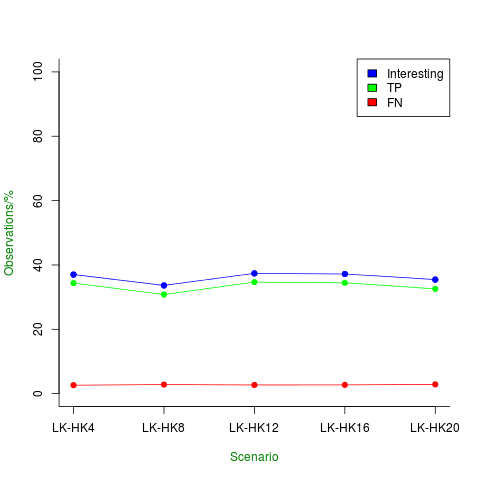
\includegraphics[width=\textwidth]{Chap7/figures/khas_int_percent.png}
% \caption{Percentage of Interesting Observations in MK-HK Variations}
% \label{fig:khas_int_percent}
% \end{figure}

% \begin{figure}[!h]
% \centering
% 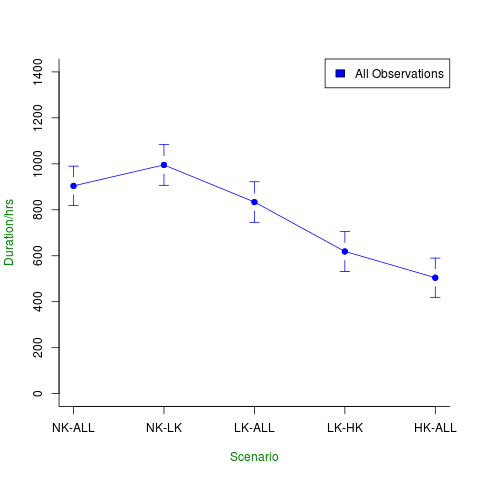
\includegraphics[width=\textwidth]{Chap7/figures/all_total.png}
% \caption{Mean Duration for All Observations in Zigbee Scenarios}
% \label{fig:all_total}
% \end{figure}

% \subsection{Unrestricted Transmission Speeds}
% In this section, we manipulated the variables set in out original simulations, that were based on existing sensed data, to identify bottlenecks that prevented observations from being received immediately. Zigbee has a low transmission rate, of 2.77 Kbps, therefore we expected increasing the transmission rate of all nodes in the network to a rate in the thousands (61920 Kbps) to determine whether this would reduce the mean transmission time for all images. Figure \ref{fig:unres_int} shows that, when compared with Figure \ref{fig:all_int}, the transmission time is reduced in all scenarios, by up to half in some cases. HK-ALL shows that this increase allows for interesting observations to be delivered with almost no delay, in near real-time. However, with a rate that should allow almost all observations to be sent in a matter of seconds, many scenarios still have a delay of 600 hours. Figure \ref{fig:unres_total} shows the average duration for all observations received at the central node and, with Wi-Fi transmission rates, we expected this to be much higher. However, when compared with Figure \ref{fig:all_total}, which shows the average duration for all observations using Zigbee as the transmission medium, we can see that the transmission time for most scenarios reduces to fewer than 500 hours. HK-ALL, remains much the same, despite the faster transmission rate. 

% Another bottleneck that we identified was the duration that each node would check for new observations, and process them. In the current solution, sensing nodes check every 10 minutes and routing nodes check every 5. This delay could cause an observation to not be picked up immediately, as well as the transmission delay. To test this, we reduced the Sensing node check to every minute and the Routing node to check every 30 seconds for new observations. Using Zigbee, the mean transmission time for all observations, in the HK-ALL scenario, was 501.02 hours. Using the increased transmission rate, it was 354.34 hours and with the reduced checking delay, the time dropped to 1.58 hours. Therefore, in order to create a real time implementation of these scenarios, one would need to use a fast transmission medium, such as Wi-Fi, and increase the time delay to check for new data; both of which would reduce the battery life of the node. This solution would ensure that all sensed data would be received almost as soon as it was captured, however, our HK-ALL Zigbee implementation would deliver interesting images within 3 hours but conserve battery life by using a radio with less power consumption and checking for new data less often. This faster solution would be primarily suited to deployments where power is not a constraint, but the real-time receipt of all sensed data is.

% \begin{figure}[!h]
% \centering
% 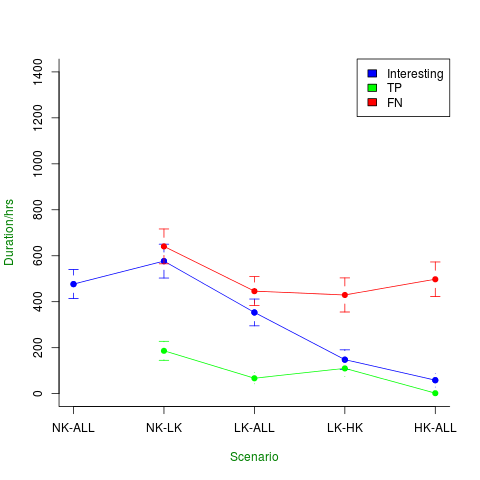
\includegraphics[width=\textwidth]{Chap7/figures/unres_all_int.png}
% \caption{Mean Duration for Interesting Observations in Unrestricted Scenarios}
% \label{fig:unres_int}
% \end{figure}

% \begin{figure}[!h]
% \centering
% 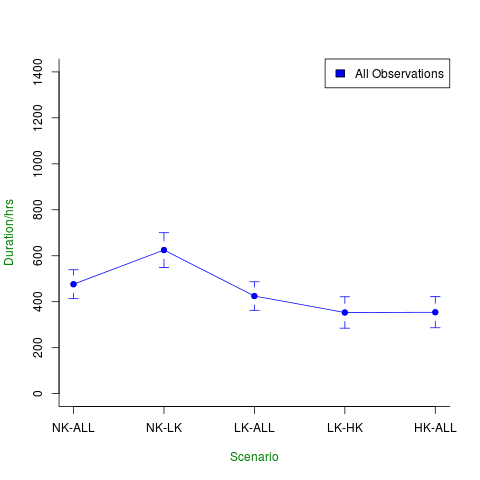
\includegraphics[width=\textwidth]{Chap7/figures/unres_all_total.png}
% \caption{Mean Duration for All Observations in Unrestricted Scenarios}
% \label{fig:unres_total}
% \end{figure}

\section{Conclusion} \label{sim:conc}
	
In this chapter, we have detailed the development of simulations to show the different scenarios for pushing knowledge out to the edge of a network. Using different levels of knowledge processing capabilities on nodes, we have shown that a network with HK processing capabilities can detect and prioritise interesting images, while simultaneously delaying empty images for a time when the network is not busy. However, using a network that solely comprises of HK nodes results in a battery life that lasts for 3 weeks on each node. The MK-HK network architecture we have proposed provides a combination of HK and MK nodes, distributed based on their role in the network. For example, nodes tasked with sensing and forwarding images only have MK processing capabilities. These simulations have shown that the HK-MK scenario results in a delay of interesting image delivery, when compared to MK-ALL, but the percentage of interesting images delivered is significantly increased.

Using a model of real world transmission rates, we have seen that the variation in transmission times can be quite large, but the difference between MK-HK and HK-ALL is not that great. This suggests that our MK-HK proposal (K-HAS) is the best solution for most scenarios as it provides a longer network lifetime with same ratio of TP:FN images as a network where every node is equipped with HK.

While the simulation is not feature complete, it is accurate enough to show how MK-HK utilises the knowledge-processing capabilities at each tier to process, and prioritise, sensed data based on knowledge gained from the environment, previously sensed data and from humans using the network. Our results also show that the difference between MK-HK and HK-ALL is  not significant enough to warrant the loss in network lifetime. However, not every scenario would be suited to this. NK-MK shows a slightly faster transmission time and a much longer network lifetime, as most nodes would not have any processing power. While the processing of sensed data would not be enough to rely on, it could act as pre-processing that could be processed further once power is not an issue. This would be well suited for networks where nodes have limited power and are not easily accessible, such as bird nest monitoring networks. 

MK-HK allows sensed data to be processed, and delivered, in near real-time with approximately 82\% of all interesting data being correctly classified. This number could increase the longer that the network is deployed, which is something we would like to investigate in the future.

Finally, we simulated the situation where there is more sensed data than the bandwidth available. The greater knowledge-processing capabilities of HK-ALL scenarios ensured that empty images were delayed and interesting observations were sent with a greater priority. While there were interesting observations misclassified as empty that were delayed, they made up less than 10\% of all interesting observations. MK-HK did receive fewer interesting observations, most likely due to its limited ability to prioritise sensed data right from the edge of the network, but the majority of interesting observations were true positives and they were prioritised over empty observations. MK-ALL, with a longer network lifetime of MK-HK and HK-ALL, did not prioritise interesting over empty data effectively but still provided more true positives than false negatives.

We can conclude that, for a power efficient WSN, the results from these simulations suggest that MK-HK can deliver many of the same benefits that HK-ALL provides while not pushing HK to the edge of the network, reducing the network lifetime. If power was of no concern, HK-ALL is able to deliver more interesting observations and prioritise more accurately from the edge of the network, as well as filtering important data more effectively when the network is saturated.







































